\documentclass{book}
\usepackage{fontspec}
\setmainfont{STIX Two Text}

%PACKAGES
\iffalse
Here are the packages that I use
\fi

\usepackage{blindtext, hyperref, verbatim, minted, graphicx, amssymb, textcomp, enumerate, tcolorbox, newunicodechar, textgreek, wasysym, tipa, eso-pic, lipsum, bbold, dsfont}
\usepackage[margin=1.3in]{geometry}
\usepackage{longtable}
\usepackage{newunicodechar}
\usepackage{amsthm}
\usepackage{tikz}
\usepackage{tikz-cd}






%ENVIRONMENTS

%Here I define some common environments. I use definitions, theorems, examples, and lemmas.


\theoremstyle{definition}
\newtheorem{definition}{Definition}
\newtheorem{theorem}{Theorem}
\newtheorem{example}{Example}
\newtheorem{lemma}{Lemma}


\newunicodechar{ₙ}{${}_{n}$}

\newunicodechar{𝓓}{$\mathcal{D}$}
\newunicodechar{∂}{$\partial$}

%\newunicodechar{π⃗}{$\stackrel{\arr}{\pi}$}

\newunicodechar{×}{$\times$}
\newunicodechar{→}{$\rightarrow$}
\newunicodechar{⟨}{$\langle$}
\newunicodechar{⟩}{$\rangle$}
\newunicodechar{↦}{$\mapsto$}
\newunicodechar{∧}{$\wedge$}
\newunicodechar{∨}{$\vee$}
\newunicodechar{∃}{$\exists$}
\newunicodechar{∀}{$\forall$}
\newunicodechar{¬}{$\neg$}
\newunicodechar{ᵃ}{${}^{\texttt{a}}$}
\newunicodechar{ᵇ}{${}^{\texttt{b}}$}
\newunicodechar{ᶜ}{${}^{\texttt{c}}$}
\newunicodechar{ᵈ}{${}^{\texttt{d}}$}
\newunicodechar{ᵉ}{${}^{\texttt{e}}$}
\newunicodechar{ᶠ}{${}^{\texttt{f}}$}
\newunicodechar{ᵍ}{${}^{\texttt{g}}$}
\newunicodechar{ʰ}{${}^{\texttt{h}}$}
\newunicodechar{ⁱ}{${}^{\texttt{i}}$}
\newunicodechar{ʲ}{${}^{\texttt{j}}$}
\newunicodechar{ᵏ}{${}^{\texttt{k}}$}
\newunicodechar{ˡ}{${}^{\texttt{l}}$}
\newunicodechar{ᵐ}{${}^{\texttt{m}}$}
\newunicodechar{ⁿ}{${}^{\texttt{n}}$}
\newunicodechar{ᵒ}{${}^{\texttt{o}}$}
\newunicodechar{ᵖ}{${}^{\texttt{ω}}$}
\newunicodechar{ʳ}{${}^{\texttt{r}}$}
\newunicodechar{ˢ}{${}^{\texttt{s}}$}
\newunicodechar{ᵗ}{${}^{\texttt{t}}$}
\newunicodechar{ᵘ}{${}^{\texttt{u}}$}
\newunicodechar{ᵛ}{${}^{\texttt{v}}$}
\newunicodechar{ʷ}{${}^{\texttt{w}}$}
\newunicodechar{ˣ}{${}^{\texttt{x}}$}
\newunicodechar{ʸ}{${}^{\texttt{y}}$}
\newunicodechar{ᶻ}{${}^{\texttt{z}}$}
\newunicodechar{⁰}{${}^{\texttt{0}}$}
\newunicodechar{¹}{${}^{\texttt{1}}$}
\newunicodechar{²}{${}^{\texttt{2}}$}
\newunicodechar{³}{${}^{\texttt{3}}$}
\newunicodechar{⁴}{${}^{\texttt{4}}$}
\newunicodechar{⁵}{${}^{\texttt{5}}$}
\newunicodechar{⁶}{${}^{\texttt{6}}$}
\newunicodechar{⁷}{${}^{\texttt{7}}$}
\newunicodechar{⁸}{${}^{\texttt{8}}$}
\newunicodechar{⁹}{${}^{\texttt{9}}$}
\newunicodechar{⁻}{${}^{\texttt{-}}$}
\newunicodechar{ᵒ}{${}^{\texttt{o}}$}
\newunicodechar{ᵖ}{${}^{\texttt{ω}}$}
\newunicodechar{⁻}{${}^{\texttt{-}}$}
\newunicodechar{¹}{${}^{\texttt{1}}$}
\newunicodechar{₀}{${}_{\texttt{0}}$}
\newunicodechar{₁}{${}_{\texttt{1}}$}
\newunicodechar{₂}{${}_{\texttt{2}}$}
\newunicodechar{₃}{${}_{\texttt{3}}$}
\newunicodechar{₄}{${}_{\texttt{4}}$}
\newunicodechar{₅}{${}_{\texttt{5}}$}
\newunicodechar{₆}{${}_{\texttt{6}}$}
\newunicodechar{₇}{${}_{\texttt{7}}$}
\newunicodechar{₈}{${}_{\texttt{8}}$}
\newunicodechar{₉}{${}_{\texttt{9}}$}
\newunicodechar{𝔸}{$\mathbb{A}$}
\newunicodechar{𝔹}{$\mathbb{B}$}
\newunicodechar{ℂ}{$\mathbb{C}$}
\newunicodechar{𝔻}{$\mathbb{D}$}
\newunicodechar{𝔼}{$\mathbb{E}$}
\newunicodechar{𝔽}{$\mathbb{F}$}
\newunicodechar{𝔾}{$\mathbb{G}$}
\newunicodechar{ℍ}{$\mathbb{H}$}
\newunicodechar{𝕀}{$\mathbb{I}$}
\newunicodechar{𝕁}{$\mathbb{J}$}
\newunicodechar{𝕂}{$\mathbb{K}$}
\newunicodechar{𝕃}{$\mathbb{L}$}
\newunicodechar{𝕄}{$\mathbb{M}$}
\newunicodechar{ℕ}{$\mathbb{N}$} 
\newunicodechar{𝕆}{$\mathbb{O}$}
\newunicodechar{ℙ}{$\mathbb{P}$}
\newunicodechar{ℚ}{$\mathbb{Q}$}
\newunicodechar{ℝ}{$\mathbb{R}$}
\newunicodechar{𝕊}{$\mathbb{S}$}
\newunicodechar{𝕋}{$\mathbb{T}$} 
\newunicodechar{𝕌}{$\mathbb{U}$}
\newunicodechar{𝕍}{$\mathbb{V}$}
\newunicodechar{𝕎}{$\mathbb{W}$}
\newunicodechar{𝕏}{$\mathbb{X}$}
\newunicodechar{𝕐}{$\mathbb{Y}$}
\newunicodechar{ℤ}{$\mathbb{Z}$}
\newunicodechar{𝕒}{$\mathbb{a}$}
\newunicodechar{𝕓}{$\mathbb{b}$}
\newunicodechar{𝕔}{$\mathbb{c}$}
\newunicodechar{𝕕}{$\mathbb{d}$}
\newunicodechar{𝕖}{$\mathbb{e}$}
\newunicodechar{𝕗}{$\mathbb{f}$}
\newunicodechar{𝕘}{$\mathbb{g}$}
\newunicodechar{𝕙}{$\mathbb{h}$}
\newunicodechar{𝕚}{$\mathbb{i}$}
\newunicodechar{𝕛}{$\mathbb{j}$}
\newunicodechar{𝕜}{$\mathbb{k}$}%𝔸𝔹ℂ𝔻𝔼𝔽𝔾ℍ𝕀𝕁𝕂𝕃𝕄ℕ𝕆ℙℚℝ𝕊𝕋𝕌𝕍𝕎𝕏𝕐ℤ𝕒𝕓𝕔𝕕𝕖𝕗𝕘𝕙𝕚𝕛𝕜𝕝𝕞𝕟𝕠𝕡𝕢𝕣𝕤𝕥𝕦𝕧𝕨𝕩𝕪𝕫
\newunicodechar{𝕝}{$\mathbb{l}$} 
\newunicodechar{𝕞}{$\mathbb{m}$}
\newunicodechar{𝕟}{$\mathbb{n}$}
\newunicodechar{𝕠}{$\mathbb{o}$}
\newunicodechar{𝕡}{$\mathbb{p}$}
\newunicodechar{𝕢}{$\mathbb{q}$}
\newunicodechar{𝕣}{$\mathbb{r}$}
\newunicodechar{𝕤}{$\mathbb{s}$}
\newunicodechar{𝕥}{$\mathbb{t}$}
\newunicodechar{𝕦}{$\mathbb{u}$}
\newunicodechar{𝕧}{$\mathbb{v}$}
\newunicodechar{𝕨}{$\mathbb{w}$}
\newunicodechar{𝕩}{$\mathbb{x}$}
\newunicodechar{𝕪}{$\mathbb{y}$}
\newunicodechar{𝕫}{$\mathbb{z}$}
\newunicodechar{𝚫}{$\Delta$}
\newunicodechar{ʃ}{$\int$}
\newunicodechar{∪}{$\cup$}
\newunicodechar{∩}{$\cap$}
\newunicodechar{±}{$\pm$}
\newunicodechar{𝔄}{$\mathfrak{A}$}




\newunicodechar{𝔅}{$\mathfrak{B}$}
\newunicodechar{ℭ}{$\mathfrak{C}$}
\newunicodechar{𝔇}{$\mathfrak{D}$}
\newunicodechar{𝔈}{$\mathfrak{E}$}
\newunicodechar{𝔉}{$\mathfrak{F}$}
\newunicodechar{𝔊}{$\mathfrak{G}$}
\newunicodechar{ℌ}{$\mathfrak{H}$}
\newunicodechar{ℑ}{$\mathfrak{I}$}
\newunicodechar{𝔍}{$\mathfrak{J}$}
\newunicodechar{𝔎}{$\mathfrak{K}$}
\newunicodechar{𝔏}{$\mathfrak{L}$}
\newunicodechar{𝔐}{$\mathfrak{M}$}
\newunicodechar{𝔑}{$\mathfrak{N}$}
\newunicodechar{𝔒}{$\mathfrak{O}$}
\newunicodechar{𝔓}{$\mathfrak{P}$}
\newunicodechar{𝔔}{$\mathfrak{Q}$}
\newunicodechar{ℜ}{$\mathfrak{R}$}
\newunicodechar{𝔖}{$\mathfrak{S}$}
\newunicodechar{𝔗}{$\mathfrak{T}$}
\newunicodechar{𝔘}{$\mathfrak{U}$}
\newunicodechar{𝔙}{$\mathfrak{V}$}
\newunicodechar{𝔚}{$\mathfrak{W}$}
\newunicodechar{𝔛}{$\mathfrak{X}$}
\newunicodechar{𝔜}{$\mathfrak{Y}$}
\newunicodechar{ℨ}{$\mathfrak{Z}$}

\newunicodechar{𝔞}{$\mathfrak{a}$}
\newunicodechar{𝔟}{$\mathfrak b$}
\newunicodechar{𝔠}{$\mathfrak{c}$}
\newunicodechar{𝔡}{$\mathfrak{d}$}
\newunicodechar{𝔢}{$\mathfrak{e}$}
\newunicodechar{𝔣}{$\mathfrak{f}$}
\newunicodechar{𝔤}{$\mathfrak{g}$}
\newunicodechar{𝔥}{$\mathfrak{h}$}
\newunicodechar{𝔦}{$\mathfrak{i}$}
\newunicodechar{𝔧}{$\mathfrak{j}$}
\newunicodechar{𝔨}{$\mathfrak{k}$}
\newunicodechar{𝔩}{$\mathfrak{l}$}
\newunicodechar{𝔪}{$\mathfrak{m}$}
\newunicodechar{𝔫}{$\mathfrak{n}$}
\newunicodechar{𝔬}{$\mathfrak{o}$}
\newunicodechar{𝔭}{$\mathfrak{ω}$}
\newunicodechar{𝔮}{$\mathfrak{q}$}
\newunicodechar{𝔯}{$\mathfrak{r}$}
\newunicodechar{𝔰}{$\mathfrak{s}$}
\newunicodechar{𝔱}{$\mathfrak{t}$}
\newunicodechar{𝔲}{$\mathfrak{u}$}
\newunicodechar{𝔳}{$\mathfrak{v}$}
\newunicodechar{𝔴}{$\mathfrak{w}$}
\newunicodechar{𝔵}{$\mathfrak{x}$}
\newunicodechar{𝔶}{$\mathfrak{y}$}
\newunicodechar{𝔷}{$\mathfrak{z}$}

\newunicodechar{𝐀}{${\bf{A}}$}
\newunicodechar{𝐁}{${\bf{B}}$}
\newunicodechar{𝐂}{${\bf{C}}$}
\newunicodechar{𝐃}{${\bf{D}}$}
\newunicodechar{𝐄}{${\bf{E}}$}
\newunicodechar{𝐅}{${\bf{F}}$}
\newunicodechar{𝐆}{${\bf{G}}$}
\newunicodechar{𝐇}{${\bf{H}}$}
\newunicodechar{𝐈}{${\bf{I}}$}
\newunicodechar{𝐉}{${\bf{J}}$}
\newunicodechar{𝐊}{${\bf{K}}$}
\newunicodechar{𝐋}{${\bf{L}}$}
\newunicodechar{𝐌}{${\bf{M}}$}
\newunicodechar{𝐍}{${\bf{N}}$}
\newunicodechar{𝐎}{${\bf{O}}$}
\newunicodechar{𝐏}{${\bf{P}}$}
\newunicodechar{𝐐}{${\bf{Q}}$}
\newunicodechar{𝐑}{${\bf{R}}$}
\newunicodechar{𝐒}{${\bf{S}}$}
\newunicodechar{𝐓}{${\bf{T}}$}
\newunicodechar{𝐔}{${\bf{U}}$}
\newunicodechar{𝐕}{${\bf{V}}$}
\newunicodechar{𝐖}{${\bf{W}}$}
\newunicodechar{𝐗}{${\bf{X}}$}
\newunicodechar{𝐘}{${\bf{Y}}$}
\newunicodechar{𝐙}{${\bf{Z}}$}

\newunicodechar{𝐚}{${\bf{a}}$}
\newunicodechar{𝐛}{${\bf{b}}$}
\newunicodechar{𝐜}{${\bf{c}}$}
\newunicodechar{𝐝}{${\bf{d}}$}
\newunicodechar{𝐞}{${\bf{e}}$}
\newunicodechar{𝐟}{${\bf{f}}$}
\newunicodechar{𝐠}{${\bf{g}}$}
\newunicodechar{𝐡}{${\bf{h}}$}
\newunicodechar{𝐢}{${\bf{i}}$}
\newunicodechar{𝐣}{${\bf{j}}$}
\newunicodechar{𝐤}{${\bf{k}}$}
\newunicodechar{𝐥}{${\bf{l}}$}
\newunicodechar{𝐦}{${\bf{m}}$}
\newunicodechar{𝐧}{${\bf{n}}$}
\newunicodechar{𝐨}{${\bf{o}}$}
\newunicodechar{𝐩}{${\bf{ω}}$}
\newunicodechar{𝐪}{${\bf{q}}$}
\newunicodechar{𝐫}{${\bf{r}}$}
\newunicodechar{𝐬}{${\bf{s}}$}
\newunicodechar{𝐭}{${\bf{t}}$}
\newunicodechar{𝐮}{${\bf{u}}$}
\newunicodechar{𝐯}{${\bf{v}}$}
\newunicodechar{𝐰}{${\bf{w}}$}
\newunicodechar{𝐱}{${\bf{x}}$}
\newunicodechar{𝐲}{${\bf{y}}$}
\newunicodechar{𝐳}{${\bf{z}}$}

\newunicodechar{⊣}{\ensuremath{\dashv}}
\newunicodechar{ॱ}{${}^{\cdot}$}
\newunicodechar{𛲔}{${}_{\cdot}$}
\newunicodechar{⋯}{$\cdots$}
\newunicodechar{⇄}{$\rightleftarrows$}
\newunicodechar{⇆}{$\leftrightarrows$}

\newunicodechar{ꜝ}{$\raisebox{1ex}{\scalebox{0.5}{\texttt{!}}}$}
\newunicodechar{ꜞ}{$\raisebox{1ex}{\scalebox{0.5}{\texttt{¡}}}$}



%This is notation we will use for categories


\newunicodechar{𝟙}{$\mathbb{1}$}
\newunicodechar{∘}{$\circ$}

%This is notation we will use for twocategories


\newunicodechar{𝟏}{${\bold{1}}$}
\newunicodechar{⭢}{$\longrightarrow$}
\newunicodechar{•}{${\bullet}$}
\newunicodechar{∙}{${\bullet}$}

%This is notation we will use for ∞-ℂ𝕒𝕥

\newunicodechar{よ}{$
\includegraphics[width=0.27cm,height=0.27cm]{yon.png}$}
\newunicodechar{⊥}{$\bot$}
\newunicodechar{∼}{$\sim$}
\newunicodechar{≃}{$\simeq$}
\newunicodechar{≅}{$\cong$}
\newunicodechar{∞}{$\infty$}

\newunicodechar{α}{$\alpha$}
\newunicodechar{β}{$\beta$}
\newunicodechar{γ}{$\gamma$}
\newunicodechar{δ}{$\delta$}
\newunicodechar{ε}{$\epsilon$}
\newunicodechar{η}{$\eta$}
\newunicodechar{ζ}{$\zeta$}
\newunicodechar{θ}{$\theta$}
\newunicodechar{ι}{$\iota$}
\newunicodechar{μ}{$\mu$}
\newunicodechar{κ}{$\kappa$}
\newunicodechar{λ}{$\lambda$}
\newunicodechar{ρ}{$\rho$}
\newunicodechar{π}{$\pi$}
\newunicodechar{σ}{$\sigma$}
\newunicodechar{τ}{$\tau$}
\newunicodechar{υ}{$\upsilon$}
\newunicodechar{φ}{$\phi$}
\newunicodechar{ψ}{$\psi$}
\newunicodechar{ξ}{$\xi$}
\newunicodechar{χ}{$\chi$}
\newunicodechar{ω}{$\omega$}

\newunicodechar{⊗}{$\otimes$}

\makeatletter
\newcommand*{\shifttext}[2]{\settowidth{\@tempdima}{#2}\makebox[\@tempdima]{\hspace*{#1}#2}}
\makeatother
\definecolor{Red}{cmyk}{0.1, 0.70, 0.65, 0.00, 1.00}
\definecolor{Blue}{cmyk}{0.9, 0.2, 0.2, 0.00, 1.00}
\definecolor{Yellow}{cmyk}{0.0, 0.00, 0.7, 0.00, 0.5}
\definecolor{Green}{cmyk}{0.6, 0.0, 0.6, 0.00, 1.00}
\definecolor{Purple}{cmyk}{0.8, 0.3, 0.3, 0.00, 1.00}
\definecolor{Orange}{cmyk}{0.0, 0.3, 0.7, 0.00, 1.00}
\definecolor{Grey}{cmyk}{0.13, 0.13, 0.13, 0.00, 1.00}
\newcounter{definitioncounter}
\setcounter{definitioncounter}{1}
\newcounter{theoremcounter}
\setcounter{theoremcounter}{1}
\newcounter{printcounter}
\setcounter{printcounter}{1}
\newcounter{examplecounter}
\setcounter{examplecounter}{1}
\newcounter{ccounter}
\setcounter{ccounter}{1}
\newcounter{pcounter}
\setcounter{pcounter}{1}
\newcounter{lcounter}
\setcounter{lcounter}{1}
\newcounter{sectioncount}
\newcounter{subsectioncount}
\setcounter{sectioncount}{1}
\renewcommand{\section}[1]{\newpage\ \\ \ \\ \begin{center} \scalebox{1.5}{\texttt{\thesectioncount . #1}} \stepcounter{sectioncount} \setcounter{subsectioncount}{1} \end{center} \begin{center} \ \\ \ \\ \thispagestyle{empty} \end{center}}
\renewcommand{\subsection}[1]{\texttt{\thesubsectioncount . #1} \stepcounter{subsectioncount}}
\renewcommand{\backslash}{\reflectbox{\texttt{/}}}

\newcounter{chaptercount}
\renewcommand{\chapter}[1]{
\newpage
{
\Huge 
\begin{center}
\ \\
\ \\
\thispagestyle{empty}
\texttt{#1}
\end{center}}
\ \\
\ \\
}

\newcounter{partcount}
\stepcounter{partcount}
\renewcommand{\part}[1]{
\newpage
{
\Huge 
\begin{center}
\ \\
\ \\
\ \\
\ \\
\ \\
\ \\
\thispagestyle{empty}
\texttt{PART {\thepartcount}: #1}
\stepcounter{partcount}
\end{center}}
\ \\
\ \\
}
\begin{document}

\thispagestyle{empty} 

\AddToShipoutPicture*
    {\put(540,720){

    \href{http://www.linearlibrary.net}{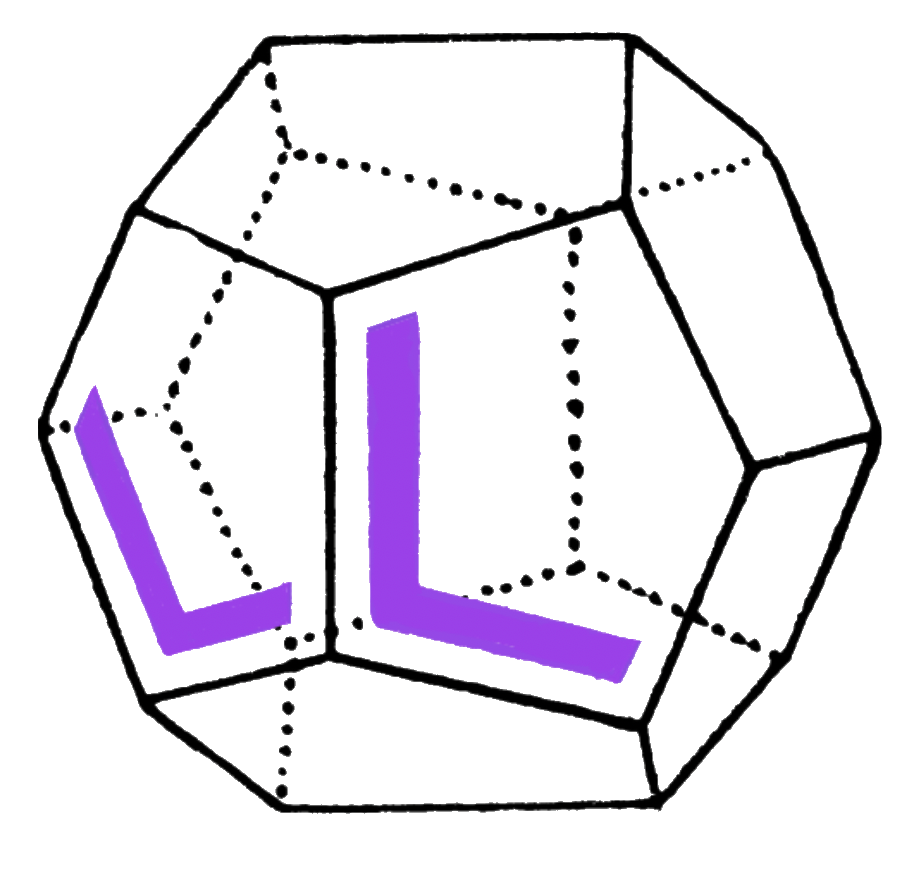
\includegraphics[width=2cm,height=2cm]{ll.png}}

    }}

\AddToShipoutPicture*
  {\put(470,767){
    \href{https://github.com/linlib/CategoriesandHilbertSpaces/StringDiagramGenerator.py}{\texttt{.py file}}
  }}

\AddToShipoutPicture*
  {\put(470,752){
    \href{https://github.com/linlib/ThreeWhiteheadTheoremsandThreePuppeSequences/ThreeWhiteheadTheoremsandThreePuppeSequences.tex}{\texttt{.tex file}}\\

  }}


\AddToShipoutPicture*
  {\put(470,737){

    \href{http://linearlibrary.net/ThreeWhiteheadTheoremsandThreePuppeSequences/ThreeWhiteheadTheoremsandThreePuppeSequences.pdf}{\texttt{.pdf file}}\\

  }}

  \AddToShipoutPicture*
  {\put(470,722){
    \href{https://github.com/linlib/ThreeWhiteheadTheoremsandThreePuppeSequences/ThreeWhiteheadTheoremsandThreePuppeSequences.lean}{\texttt{.lean file}}

  }}

\ \\

%LEAN: 
\begin{center}
\begin{tcolorbox}[width=6.4in,colback={white},coltitle=white]
\begin{center}
\ \\
\scalebox{3}{Two Theorems in Classifying Space Theory and Two Variations Each}\\
\ \\
\end{center}
\end{tcolorbox}
\end{center}
\ \\

{\footnotesize
\begin{center}
\scalebox{1.1}{
\begin{tabular}{|| l | l ||} 
\hline
\hline
E⃗ : Functor (OperadicCategory ∞-Cat) ∞-Cat & e⃗ : \{C : ∞-Cat \} → \{ D : ∞-Cat \} → (F : ∞-Cat.hom C D) → Functor (OperadicPresheaf (O⃗.obj D)) (∞-Cat⁄D)\\
\hline
B⃗ : Functor (OperadicCategory ∞-Cat) ∞-Cat & b⃗ : \{ C : ∞-Cat \} → \{ D : ∞-Cat \} → (F : ∞-Cat.hom C D) → Functor (OperadicPresheaf (O⃗.obj D)) (∞-Cat⁄D) \\
 \hline
∂⃗ : (C : OperadicCategory ∞-Cat) → ∞-Cat.hom (E⃗.obj C) (B⃗.obj C) & ∇⃗ : \{ C : ∞-Cat \} → \{ D : ∞-Cat \} → (F : ∞-Cat.hom C D) → (∞-Cat⁄D).hom (e⃗.obj F) (b⃗.obj F)\\
\hline
\hline
E⃡ : Functor (OperadicGroupoid ∞-Grpd) ∞-Grpd & e⃡ : \{ X : ∞-Cat \} → \{ Y : ∞-Cat \} → (F : ∞-Cat.hom X Y) → Functor (OperadicGroupoidAction (O⃡.obj Y)) (∞-Grpd⁄Y) \\
\hline
B⃡ : Functor (OperadicGroupoid ∞-Grpd) ∞-Grpd & b⃡ : \{ X : ∞-Grpd \} → \{ Y : ∞-Grpd \} → (F : ∞-Cat.hom X Y) → Functor (OperadicGroupoidAction (O⃡.obj Y)) (∞-Grpd⁄Y) \\
 \hline
∂⃡ : (G : OperadicCategory ∞-Grpd) → ∞-Grpd.hom (E⃡.obj G) (B⃡.obj G) & ∇⃡ : \{ X : ∞-Grpd \} → \{ Y : ∞-Grpd \} → (F : ∞-Grpd.hom X Y) → (∞-Cat⁄D).hom (e⃡.obj F) (b⃡.obj F) \\
 \hline
 \hline 
E : OperadicGroup ∞-Grpd₋₁ ⭢ ∞-Grpd₋₁ & e : \{ X₋₁ : ∞-Grpd₋₁ \} → \{ Y₋₁ : ∞-Grpd₋₁ \} → (F : ∞-Grpd₋₁.hom X₋₁ Y₋₁) → Functor (∞-Grpd₋₁⁄Y₋₁) (OperadicGroupAction (O.obj Y₋₁)) \\
\hline
B : OperadicGroup ∞-Grpd₋₁ ⭢ ∞-Grpd₋₁ & b : \{ X₋₁ : ∞-Grpd₋₁ \} → \{ Y₋₁ : ∞-Grpd₋₁ \} → (F : ∞-Grpd₋₁.hom X₋₁ Y₋₁) → Functor (∞-Grpd₋₁⁄Y₋₁) (OperadicGroupAction (O.obj Y₋₁))\\
\hline
∂ : (G₋₁ : OperadicGroup ∞-Grpd₋₁) → ∞-Grpd₋₁.hom (E.obj G₋₁) (B.obj G₋₁) & ∇ : \{ G₋₁ : ∞-Grpd₀ \} → \{ Y₀ : ∞-Grpd₀ \} → (F : ∞-Grpd₋₁.hom X₋₁ Y₋₁) → (∞-Cat⁄D).hom (e.obj F) (b.obj F)  \\
\hline
\end{tabular}}
\end{center}}

%LEAN: 
\begin{center}
\begin{tcolorbox}[width=4.13in,colback={white},coltitle=white]
\scalebox{1.5}{E. Dean Young}
\end{tcolorbox}
\end{center}

\newpage
\ \\


\section{Contents}



{
\footnotesize
\begin{longtable}{|| l || l ||} 
\hline
\multicolumn{1}{||c||}{$\texttt{Section}$} & \multicolumn{1}{|c||}{$\texttt{Description}$} \\
\hline
\hline
Unfinished & \\
\hline
Contents & \\
\hline
Unicode & \\
\hline
Introduction & \\
\hline \hline
\multicolumn{2}{||c||}{\texttt{PART I: } BASED CONNECTED ∞-GROUPOIDS} \\
\hline \hline
\multicolumn{2}{||c||}{\texttt{Chapter 1: } Operadic Groups and Operadic Group Actions} \\
\hline \hline
OperadicGroups & \\
\hline
OperadicGroupActions & \\
\hline \hline
\multicolumn{2}{||c||}{\texttt{Chapter 2: }B and E} \\
\hline \hline
E : OperadicGroup ∞-Grpd₋₁ ⭢ ∞-Grpd₋₁ &  \\
\hline
e : \{ X₋₁ : ∞-Grpd₋₁ \} → \{ Y₋₁ : ∞-Grpd₋₁ \} → (F : ∞-Grpd₋₁.hom X₋₁ Y₋₁) → Functor (∞-Grpd₋₁⁄Y₋₁) (OperadicGroupAction (O.obj Y₋₁))  & \\
\hline
B : OperadicGroup ∞-Grpd₋₁ ⭢ ∞-Grpd₋₁ &  \\
\hline
b : \{ X₋₁ : ∞-Grpd₋₁ \} → \{ Y₋₁ : ∞-Grpd₋₁ \} → (F : ∞-Grpd₋₁.hom X₋₁ Y₋₁) → Functor (∞-Grpd₋₁⁄Y₋₁) (OperadicGroupAction (O.obj Y₋₁)) & \\
\hline
∂ : (G₋₁ : OperadicGroup ∞-Grpd₋₁) → ∞-Grpd₋₁.hom (E.obj G₋₁) (B.obj G₋₁) &  \\
\hline
∇ : \{ G₋₁ : ∞-Grpd₀ \} → \{ Y₀ : ∞-Grpd₀ \} → (F : ∞-Grpd₋₁.hom X₋₁ Y₋₁) → (∞-Cat⁄D).hom (e.obj F) (b.obj F) & \\
\hline
\multicolumn{2}{||c||}{\texttt{Chapter 3: }The Recognition Theorem} \\
\hline \hline
 & \\
\hline
 & \\
\multicolumn{2}{||c||}{\texttt{Chapter 4: }The Classifying Space Theorem} \\
\hline \hline
 & \\
\hline
 & \\
\hline \hline
\multicolumn{2}{||c||}{\texttt{PART II: } ∞-GROUPOIDS} \\
\hline \hline
\multicolumn{2}{||c||}{\texttt{Chapter 5: } Operadic Groupoids and Operadic Groupoid Actions} \\
\hline \hline
OperadicGroupoids & \\
\hline 
OperadicGroupoidActions & \\
\hline \hline
\multicolumn{2}{||c||}{\texttt{Chapter 6: }B⃡ and E⃡} \\
\hline \hline
E⃡ : Functor (OperadicGroupoid ∞-Grpd) ∞-Grpd & \\
\hline
e⃡ : \{ X : ∞-Cat \} → \{ Y : ∞-Cat \} → (F : ∞-Cat.hom X Y) → Functor (OperadicGroupoidAction (O⃡.obj Y)) (∞-Grpd⁄Y) & \\
\hline
B⃡ : Functor (OperadicGroupoid ∞-Grpd) ∞-Grpd & \\
\hline
b⃡ : \{ X : ∞-Grpd \} → \{ Y : ∞-Grpd \} → (F : ∞-Cat.hom X Y) → Functor (OperadicGroupoidAction (O⃡.obj Y)) (∞-Grpd⁄Y) & \\
 \hline
∂⃡ : (G : OperadicCategory ∞-Grpd) → ∞-Grpd.hom (E⃡.obj G) (B⃡.obj G) & \\
\hline
∇⃡ : \{ X : ∞-Grpd \} → \{ Y : ∞-Grpd \} → (F : ∞-Grpd.hom X Y) → (∞-Cat⁄D).hom (e⃡.obj F) (b⃡.obj F) & \\
\hline \hline
\multicolumn{2}{||c||}{\texttt{Chapter 7: }The Recognition Theorem for ∞-Groupoids} \\
\hline \hline
 & \\
\hline
 & \\
\multicolumn{2}{||c||}{\texttt{Chapter 8: }The Classifying Space Theorem for ∞-Groupoids} \\
\hline \hline
 & \\
\hline
 & \\
\hline \hline
\multicolumn{2}{||c||}{\texttt{PART III: } ∞-CATEGORIES} \\
\hline \hline
\multicolumn{2}{||c||}{\texttt{Chapter 9: }Operadic Categories and Operadic Presheaves} \\
\hline \hline
OperadicCategory & \\
\hline
OperadicPresheaves & \\
\hline \hline
\multicolumn{2}{||c||}{\texttt{Chapter 10: }The Recognition Theorem for ∞-Categories} \\
\hline \hline
E⃗ : Functor (OperadicCategory ∞-Cat) ∞-Cat  & \\ 
\hline
e⃗ : \{C : ∞-Cat \} → \{ D : ∞-Cat \} → (F : ∞-Cat.hom C D) → Functor (OperadicPresheaf (O⃗.obj D)) (∞-Cat⁄D) & \\
\hline
B⃗ : Functor (OperadicCategory ∞-Cat) ∞-Cat & \\
\hline
b⃗ : \{ C : ∞-Cat \} → \{ D : ∞-Cat \} → (F : ∞-Cat.hom C D) → Functor (OperadicPresheaf (O⃗.obj D)) (∞-Cat⁄D) & \\
 \hline
∂⃗ : (C : OperadicCategory ∞-Cat) → ∞-Cat.hom (E⃗.obj C) (B⃗.obj C) & \\
\hline
∇⃗ : \{ C : ∞-Cat \} → \{ D : ∞-Cat \} → (F : ∞-Cat.hom C D) → (∞-Cat⁄D).hom (e⃗.obj F) (b⃗.obj F) & \\
\hline \hline
\multicolumn{2}{||c||}{\texttt{Chapter 11: }The Recognition Theorem for ∞-Categories} \\
\hline \hline
 & \\
\hline
 & \\
\hline \hline
\multicolumn{2}{||c||}{\texttt{Chapter 12: }The Classifying Space Theorem for ∞-Categories} \\
\hline \hline
 & \\
\hline
 & \\
\hline \hline
\end{longtable}
}

\chapter{Introduction}

\newpage

In ```TheWhiteheadTheoremandTwoVariations''', I will be defining six "internal" structures based on ```Galois Theories''' by Janelidze and Borceux, as well as six ```operadic''' structures 

\iffalse
{\footnotesize
\begin{center}
\scalebox{1.1}{
\begin{tabular}{|| l | l || l | l || } 
\hline
\hline
\multicolumn{2}{||c||}{Internal} & \multicolumn{2}{||c||}{Operadic} \\
\hline
\multicolumn{2}{||c||}{Unitial} & \multicolumn{2}{||c||}{Actional} & \multicolumn{2}{||c||}{Unitial} & \multicolumn{2}{||c||}{Actional} \\
\hline
\hline
$\texttt{InternalCategory : Cat → Cat}$ & $\texttt{InternalPresheaf : (C : Cat) → (InternalCategory C) → Cat}$ & $\texttt{OperadicCategory\_(-) : ∞-Cat\_(-) → ∞-Cat\_(-)}$ & OperadicPresheaf\_(-) : (X : ∞-Cat\_(-)) → ∞-Cat\_(-)}$ \\
\hline
$\texttt{InternalGroupoid\_(-) : Cat\_(-) → Cat\_(-)}$ & $\texttt{InternalGroupoidAction : (C : Cat) → (InternalGroupoid C) → Cat}$& $\texttt{OperadicGroupoid\_(-) : ∞-Cat\_(-) → ∞-Cat\_(-)}$ & OperadicGroupoidAction\_(-) : (OperadicGroupoid\_() C) → (InternalCategory C) → ∞-Cat\_(-) → ∞-Cat\_(-)}$ \\
\hline
$\texttt{InternalGroup\_(-) : Cat\_(-) → Cat\_(-)}$ & $\texttt{InternalGroupAction : (C : Cat) → (InternalGroup C) → Cat}$ & $\texttt{OperadicGroup\_(-) : ∞-Cat\_(-) → ∞-Cat\_(-)}$ & $\texttt{OperadicGroupAction}$\_$\texttt{(-) : ∞-Cat\_(-) → ∞-Cat\_(-)}$\\
 \hline
\end{tabular}}
\end{center}}
\ \\
{\footnotesize
\begin{center}
\scalebox{1.1}{
\begin{tabular}{|| l || l ||} 
\hline
\hline
Ω⃗ : ∞-Cat ⭢ ∞-Cat & ω⃗ : (C : ∞-Cat) → (D : ∞-Cat) → (F : ∞-Cat.hom C D) → (∞-Cat⁄D) ⭢ ∞-Cat \\
\hline
O⃗ : ∞-Cat ⭢ OperadicCategory ∞-Cat & o⃗ : (C : ∞-Cat) → (D : ∞-Cat) → (F : ∞-Cat.hom C D) → (∞-Cat⁄D) ⭢ OperadicPresheaf (O⃗.obj D)\\
\hline
P⃗ : ∞-Cat ⭢ InternalCategory D(∞-Cat) & p⃗ : (C : ∞-Cat) → (D : ∞-Cat) → (F : ∞-Cat.hom C D) → (∞-Cat⁄D) ⭢ InternalPresheaf (P⃗.obj D) \\
\hline
\hline
Ω⃡ : ∞-Grpd ⭢ ∞-Grpd & ω⃡ : (X : ∞-Grpd) → (Y : ∞-Grpd) → (F : ∞-Cat.hom X Y) → (∞-Grpd⁄Y) ⭢ ∞-Grpd \\
\hline
O⃡ : ∞-Grpd ⭢ OperadicGroupoid ∞-Grpd & o⃡ : (X : ∞-Grpd) → (Y : ∞-Grpd) → (F : ∞-Cat.hom X Y) → (∞-Grpd⁄Y) ⭢ OperadicGroupoidAction (O⃡.obj Y) \\
\hline
P⃡ : ∞-Grpd ⭢ InternalGroupoid D(∞-Grpd) & p⃡ : (X : ∞-Grpd) → (Y : ∞-Grpd) → (F : ∞-Cat.hom C D) → (∞-Grpd⁄Y) ⭢ InternalGroupoidAction (P⃡.obj Y)  \\
\hline
\hline
Ω : ∞-Grpd₋₁ ⭢ ∞-Grpd₋₁  & ω : (X₋₁ : ∞-Grpd₋₁) → (Y₋₁ : ∞-Grpd₋₁) → (F : ∞-Grpd₋₁.hom X₋₁ Y₋₁) → (∞-Grpd₋₁⁄Y₋₁) ⭢ ∞-Grpd₋₁ \\
\hline
O : ∞-Grpd₋₁ ⭢ OperadicGroup ∞-Grpd₋₁ & o : (X₋₁ : ∞-Grpd₋₁) → (Y₋₁ : ∞-Grpd₋₁) → (F : ∞-Grpd₋₁.hom X₋₁ Y₋₁) → (∞-Grpd₋₁⁄Y₋₁) ⭢ OperadicGroupAction (O.obj X) \\
\hline
P : ∞-Grpd₋₁ ⭢ InternalGroup D(∞-Grpd₋₁) & p : (X₋₁ : ∞-Grpd₋₁) → (Y₋₁ : ∞-Grpd₋₁) → (F : ∞-Grpd₋₁.hom X₋₁ Y₋₁) → (∞-Grpd₋₁⁄Y₋₁) ⭢ InternalGroupAction (P.obj X₋₁) \\
\hline
 \hline
\end{tabular}}
\end{center}}
\fi



\iffalse
{\footnotesize
\begin{center}
\scalebox{1.1}{
\begin{tabular}{|| l | l ||} 
\hline
\hline
E⃗ : Functor (OperadicCategory ∞-Cat) ∞-Cat & e⃗ : \{C : ∞-Cat \} → \{ D : ∞-Cat \} → (F : ∞-Cat.hom C D) → Functor (OperadicPresheaf (O⃗.obj D)) (∞-Cat⁄D)\\
\hline
B⃗ : Functor (OperadicCategory ∞-Cat) ∞-Cat & b⃗ : \{ C : ∞-Cat \} → \{ D : ∞-Cat \} → (F : ∞-Cat.hom C D) → Functor (OperadicPresheaf (O⃗.obj D)) (∞-Cat⁄D) \\
 \hline
∂⃗ : (C : OperadicCategory ∞-Cat) → ∞-Cat.hom (E⃗.obj C) (B⃗.obj C) & ∇⃗ : \{ C : ∞-Cat \} → \{ D : ∞-Cat \} → (F : ∞-Cat.hom C D) → (∞-Cat⁄D).hom (e⃗.obj F) (b⃗.obj F)\\
\hline
\hline
E⃡ : Functor (OperadicGroupoid ∞-Grpd) ∞-Grpd & e⃡ : \{ X : ∞-Cat \} → \{ Y : ∞-Cat \} → (F : ∞-Cat.hom X Y) → Functor (OperadicGroupoidAction (O⃡.obj Y)) (∞-Grpd⁄Y) \\
\hline
B⃡ : Functor (OperadicGroupoid ∞-Grpd) ∞-Grpd & b⃡ : \{ X : ∞-Grpd \} → \{ Y : ∞-Grpd \} → (F : ∞-Cat.hom X Y) → Functor (OperadicGroupoidAction (O⃡.obj Y)) (∞-Grpd⁄Y) \\
 \hline
∂⃡ : (G : OperadicCategory ∞-Grpd) → ∞-Grpd.hom (E⃡.obj G) (B⃡.obj G) & ∇⃡ : \{ X : ∞-Grpd \} → \{ Y : ∞-Grpd \} → (F : ∞-Grpd.hom X Y) → (∞-Cat⁄D).hom (e⃡.obj F) (b⃡.obj F) \\
 \hline
 \hline 
E : OperadicGroup ∞-Grpd₋₁ ⭢ ∞-Grpd₋₁ & e : \{ X₋₁ : ∞-Grpd₋₁ \} → \{ Y₋₁ : ∞-Grpd₋₁ \} → (F : ∞-Grpd₋₁.hom X₋₁ Y₋₁) → Functor (∞-Grpd₋₁⁄Y₋₁) (OperadicGroupAction (O.obj Y₋₁)) \\
\hline
B : OperadicGroup ∞-Grpd₋₁ ⭢ ∞-Grpd₋₁ & b : \{ X₋₁ : ∞-Grpd₋₁ \} → \{ Y₋₁ : ∞-Grpd₋₁ \} → (F : ∞-Grpd₋₁.hom X₋₁ Y₋₁) → Functor (∞-Grpd₋₁⁄Y₋₁) (OperadicGroupAction (O.obj Y₋₁))\\
\hline
∂ : (G₋₁ : OperadicGroup ∞-Grpd₋₁) → ∞-Grpd₋₁.hom (E.obj G₋₁) (B.obj G₋₁) & ∇ : \{ G₋₁ : ∞-Grpd₀ \} → \{ Y₀ : ∞-Grpd₀ \} → (F : ∞-Grpd₋₁.hom X₋₁ Y₋₁) → (∞-Cat⁄D).hom (e.obj F) (b.obj F)  \\
\hline
\end{tabular}}
\end{center}}
\fi





 and ```ThePuppeSequenceandTwoVariations'''. In ```InternalUniverses''', I considered straightening and unstraightening and three variations of it, which were each considered before and after the application of D(-). This made for the six diagrams depicted on page ???. In this repository, we consider the classifying space B.\\

Let F : C ⭢ D : ∞-Cat.hom C D be an ∞-functor. Given either the C-infinity presheaf in ∞-Cat/C arising from F : ∞-Cat/D or the C-infinity presheaf in ∞-Cat/D arising from Id${}_{C}$ : ∞-Cat/C, we obtain in both cases an internal presheaf in the corresponding derived category. However, not all internal categories D : InternalCategory D(∞-Cat/C) arise from \iffalse C-InfinityCategory ∞-Cat/C \fi and not all internal presheaves S : InternalPresheaf D D(∞-Cat/C) arise from C-infinity presheaves over some C-infinity category in ∞-Cat/C.\\

In ```InternalUniverses''', we showed the straightening/unstraightening categorical equivalence and three variations using the six Ω-functors and six E-functors, treating the situations before and after the application of D(-) seperately for a total of six goals.\\

In this section, we consider classifying spaces as well as a perspective about remembering information concerning a right or left adjoint applied to a particular functor or object in the following way: E and Ω and their respective five variations give  ```remembrant''' functors E-infinity and Ω-infinity, which each produce internal presheaves in respective derived categories.\\


\begin{center}
\texttt{Plans to prove three variations of the}\\
\texttt{Whitehead theorem of homotopy groups in}\\
\texttt{Lean 4, with extensive use of Mathlib 4}
\end{center}

\thispagestyle{empty}

\ \\
{\footnotesize
\begin{center}
\scalebox{1.1}{
\begin{tabular}{|| l | l | l || l | l | l ||} 
\hline
E⃗ : ∞-Cat ⭢ ∞-Cat & B⃗ : ∞-Cat ⭢ ∞-Cat & ∂⃗ : ∞-Cat ⭢ ∞-Cat & e⃗ : (C : ∞-Cat) → (D : ∞-Cat) → Adjunction D([C,∞\_(∞-Cat)]) D([D,∞\_(∞-Cat)]) & b⃗ : (C : ∞-Cat) → (D : ∞-Cat) → D([C,∞\_(∞-Cat)]) ⭢ D([D,∞\_(∞-Cat)])&  \\
\hline
E⃡ : ∞-Grpd ⭢ ∞-Grpd & B⃡ : ∞-Grpd ⭢ ∞-Grpd & ∂⃡ : ∞-Grpd ⭢ ∞-Grpd & e⃗ : (X : ∞-Grpd) → (Y : ∞-Grpd) → Adjunction D([X,∞\_(∞-Grpd)]) D([Y,∞\_(∞-Grpd)]) & b⃡ : (X : ∞-Grpd) → (Y : ∞-Grpd) → D([X,∞\_(∞-Grpd)]) ⭢ D([Y,∞\_(∞-Grpd)])&  \\
 \hline
E : ∞-Grpd₀ ⭢ ∞-Grpd₀ & B : ∞-Grpd₀ ⭢ ∞-Grpd₀  & ∂ : ∞-Grpd₀ ⭢ ∞-Grpd₀ & e : (X : ∞-Grpd₀) → (Y: ∞-Grpd₀) → Adjunction D([X,∞\_(∞-Grpd₀)]) D([Y,∞\_(∞-Grpd₀)]) & b : (X : ∞-Grpd₀) → (Y : ∞-Grpd₀) → D([X,∞\_(∞-Grpd₀)]) ⭢ D([Y,∞\_(∞-Grpd₀)]) &  \\
 \hline
\end{tabular}}
\end{center}}
 
\newpage

By the time this repository is seen to in 2025, I will have filled out a certain six operadic structures to do with ∞-categories and ∞-groupoids. Each of these structures will be made to work together with Pow {X : Type} : λ(n : ℕ),X → X. The six operadic structures are endofunctions of one of six mathematical objects, here with an option for 12 based on models A (simplicial set model) and B (point-set model).

\begin{center}
\texttt{B¹ : Functor (Pow OperadicGroup 2) ??? (Pow OperadicGroup 2) ???}
\end{center}

\begin{center}
\texttt{Bⁿ : Functor (Pow OperadicGroup 2) ??? (Pow OperadicGroup 2) ???}
\end{center}

In this repository I construct six categorical equivalences:

\begin{enumerate}
\item Between certain operadic categories and 
\item Between certain internal categories and 
\item Between certain operadic presheaves and
\item Between certain internal presheaves and
\item Between certain operadic groupoids and 
\item Between certain internal groupoids and
\item Between certain operadic groups in ??? and ???
\item Between certain internal groups and 
\item Between certain operadic group actions
\item Between certain internal group actions
\end{enumerate}

\iffalse
Continuous functions f : X ⭢ B.obj G correspond to 
\fi







\part{BASED CONNECTED ∞-GROUPOIDS}


\chapter{Operadic Groups and Operadic Group Actions}

\chapter{The Classifying Space and the Total Space}




\part{∞-GROUPOIDS}


\chapter{Operadic Groupoids and Operadic Groupoid Actions}

\chapter{The Recognition Theorem for ∞-Groupoids}

\chapter{The Classifying Space Theorem for ∞-Groupoids}






\part{∞-CATEGORIES}


\chapter{Operadic Categories and Operadic Presheaves}

\chapter{The Recognition Theorem for ∞-Categories}

\chapter{The Classifying Space Theorem for ∞-Categories}




\iffalse
contractibility of the E's:

- For a locally contractible group?

https://en.wikipedia.org/wiki/Connection_(vector_bundle)
\fi

\iffalse
Next the B can be thought of as pushing all of the information into ∞-Cat
b can be throught of as pushing information into...

MAKE SURE TO INCLUDE //
\fi


\iffalse
\chapter{ETCC Signature for linlib2024}

\begin{enumerate}
\item NDNI 
\item NDNII 
\item NDNIII 
\end{enumerate}

\begin{enumerate}
\item The linlib signature is five binary digits (Bool × Bool) × (Bool × Bool) × Bool
\item Order : λ(b : Bool × Bool) ↦ (0,0), (0,1), (1,0), (1,1) to 
\item  : 
\item 
\item The third bit is the lowest r such that the object is an (n,r)-category, (n,r)-functor, (n,r)-natural transformation, or equation between (n,r)-natural transformations. We set r = 0 or 1 throughout the project.
\item The fourth bit is "unitial vs. actional".
\item The fifth bit is "lax vs. strict" and divides up our goals based on whether D(-) has been applied.
\end{enumerate}

The table on the next page describes a certain $2^8$ goals for 2024. The full identification number for the project is given by NDb₀b₁rb₃b₄, where b₀ and b₁ are the ND number, $\texttt{r = 0, 1}$ is the filling number, here confined to 0 or 1, b₃ refers to the lax or strict nature of the type, and b₄ refers to its unitial or actional nature.\\

\fi


\begin{center}
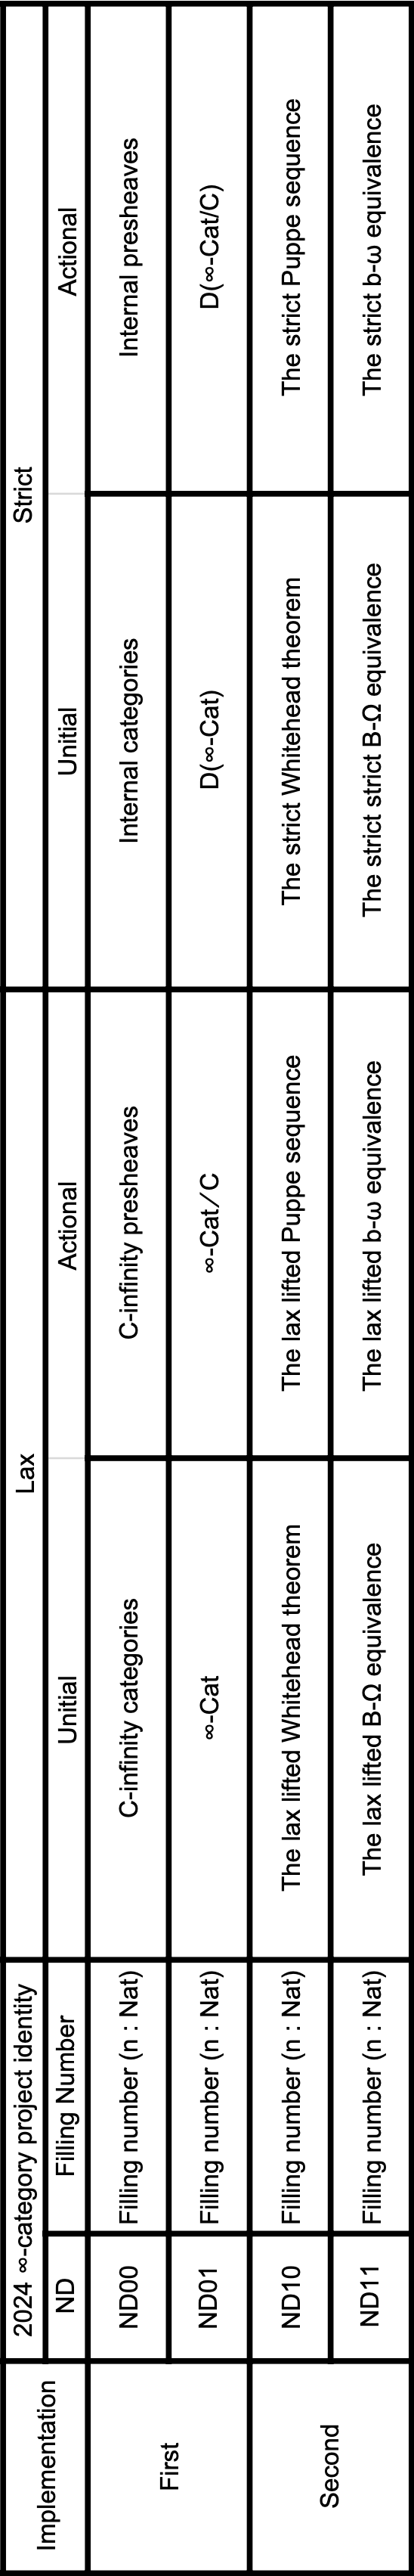
\includegraphics[width=0.24\textwidth]{mastertable.png}  \\
\end{center}
\thispagestyle{empty}

\newpage

\ \\

In ```Internal Universes''' I thought about the six variations of straightening and unstraightening featured in the diagrams below:\\


\begin{center}
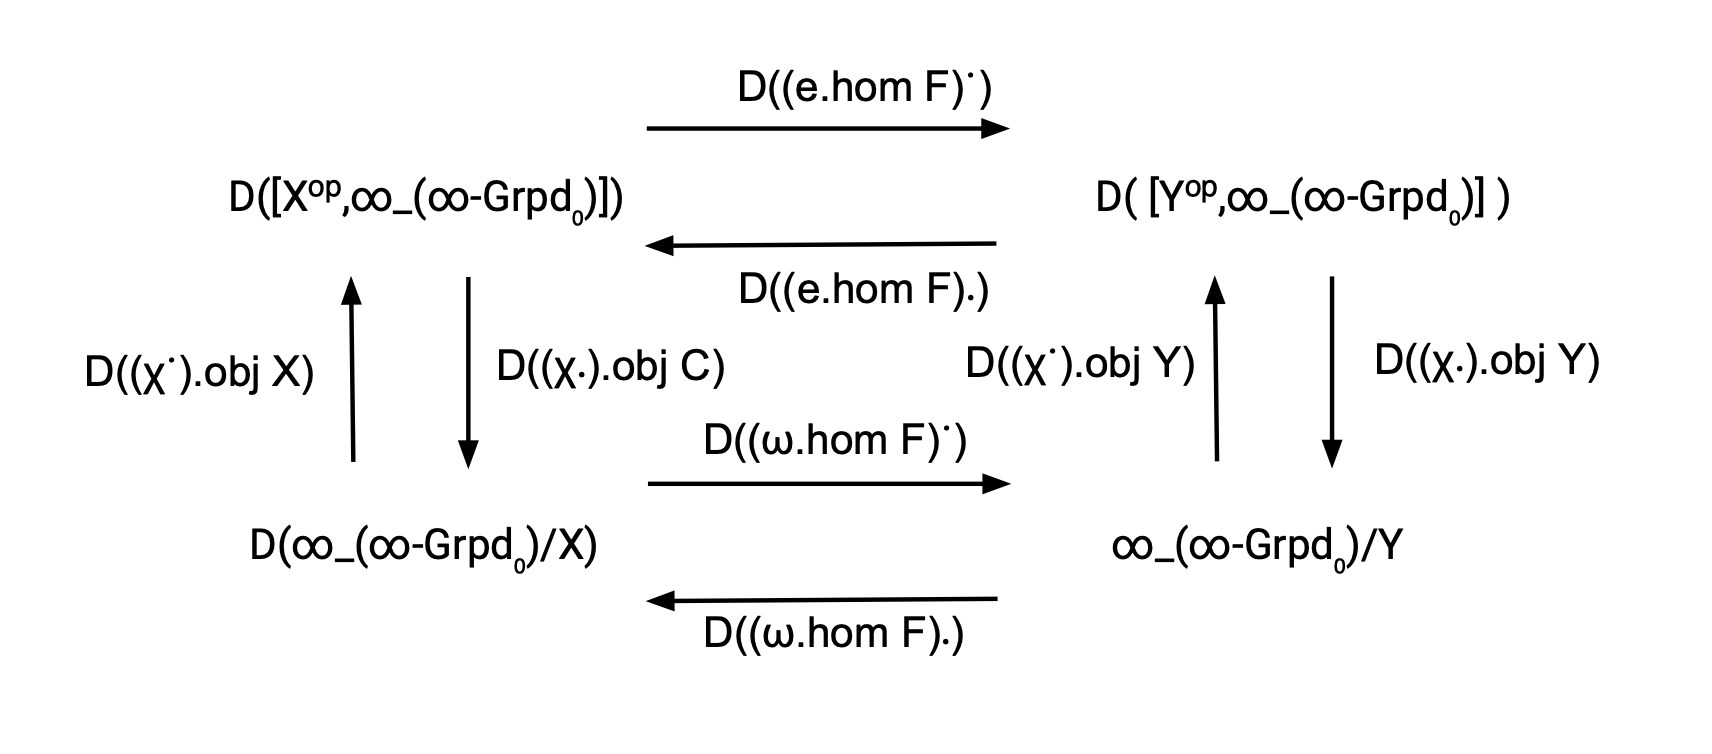
\includegraphics[width=0.9\textwidth]{ND01.png} \\
\end{center}

\ \\

\begin{center}
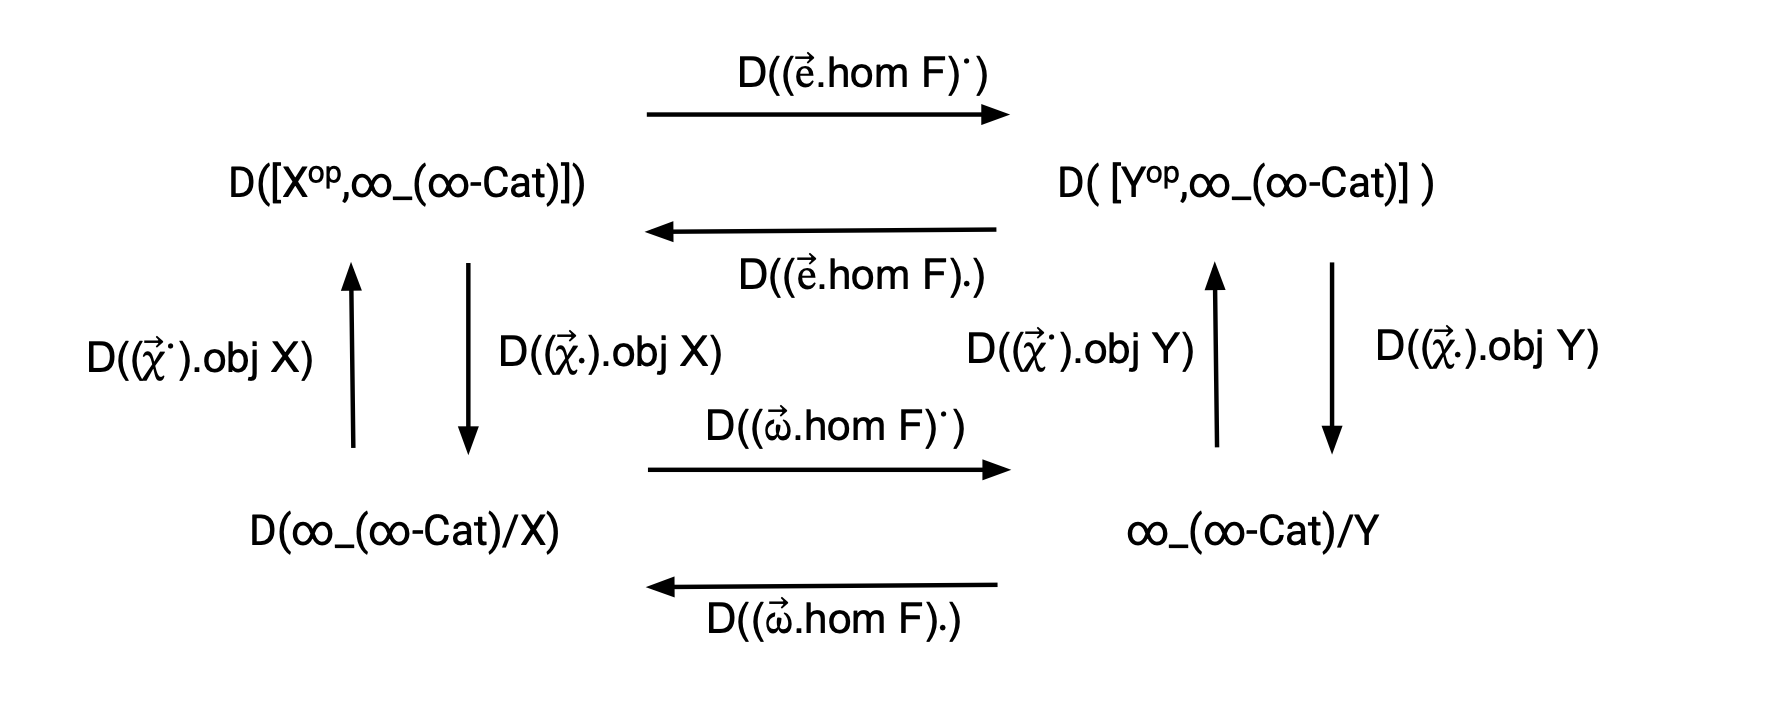
\includegraphics[width=0.9\textwidth]{ND11.png} \\
\end{center}

\ \\

\begin{center}
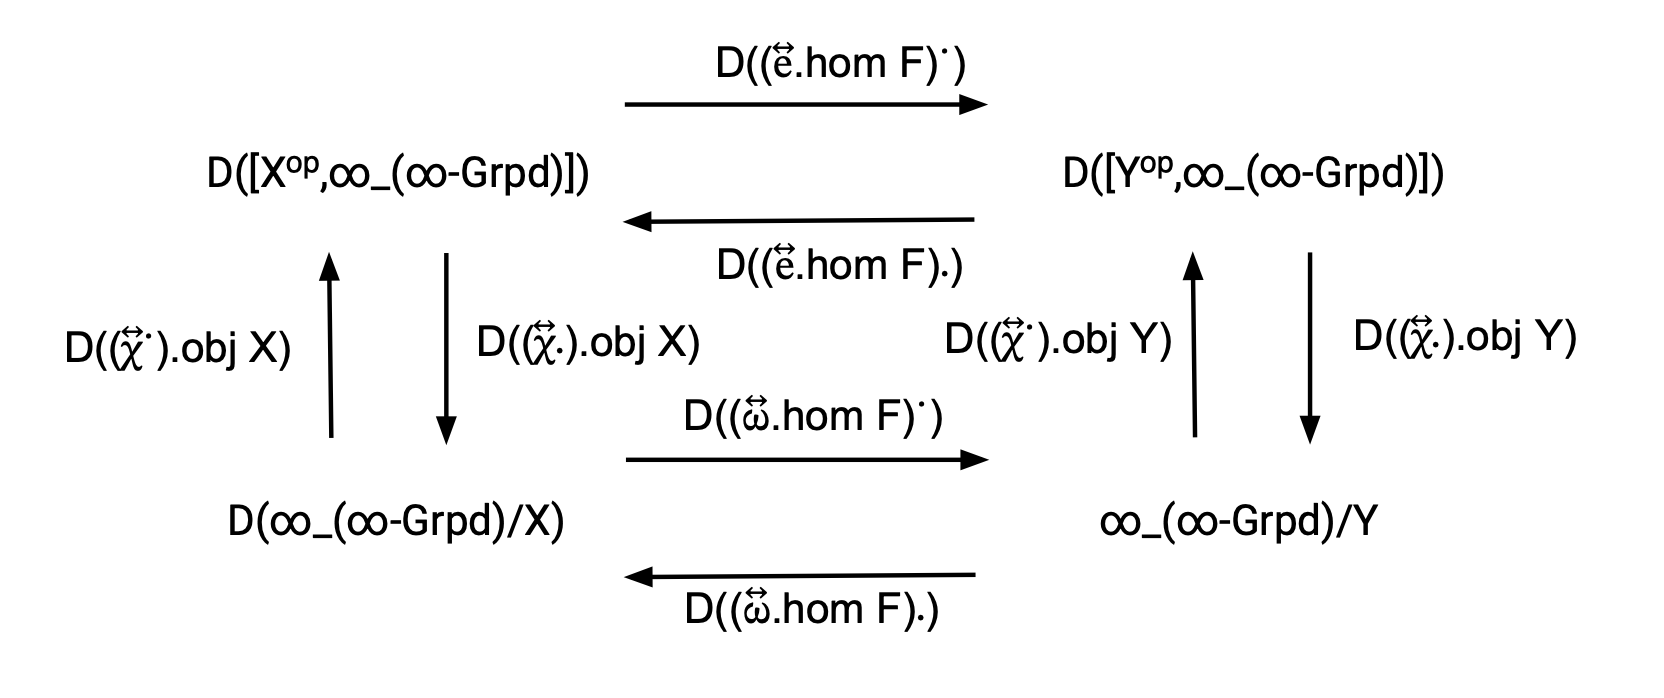
\includegraphics[width=0.9\textwidth]{ND21.png} \\
\end{center}


\newpage

\ \\

\begin{center}
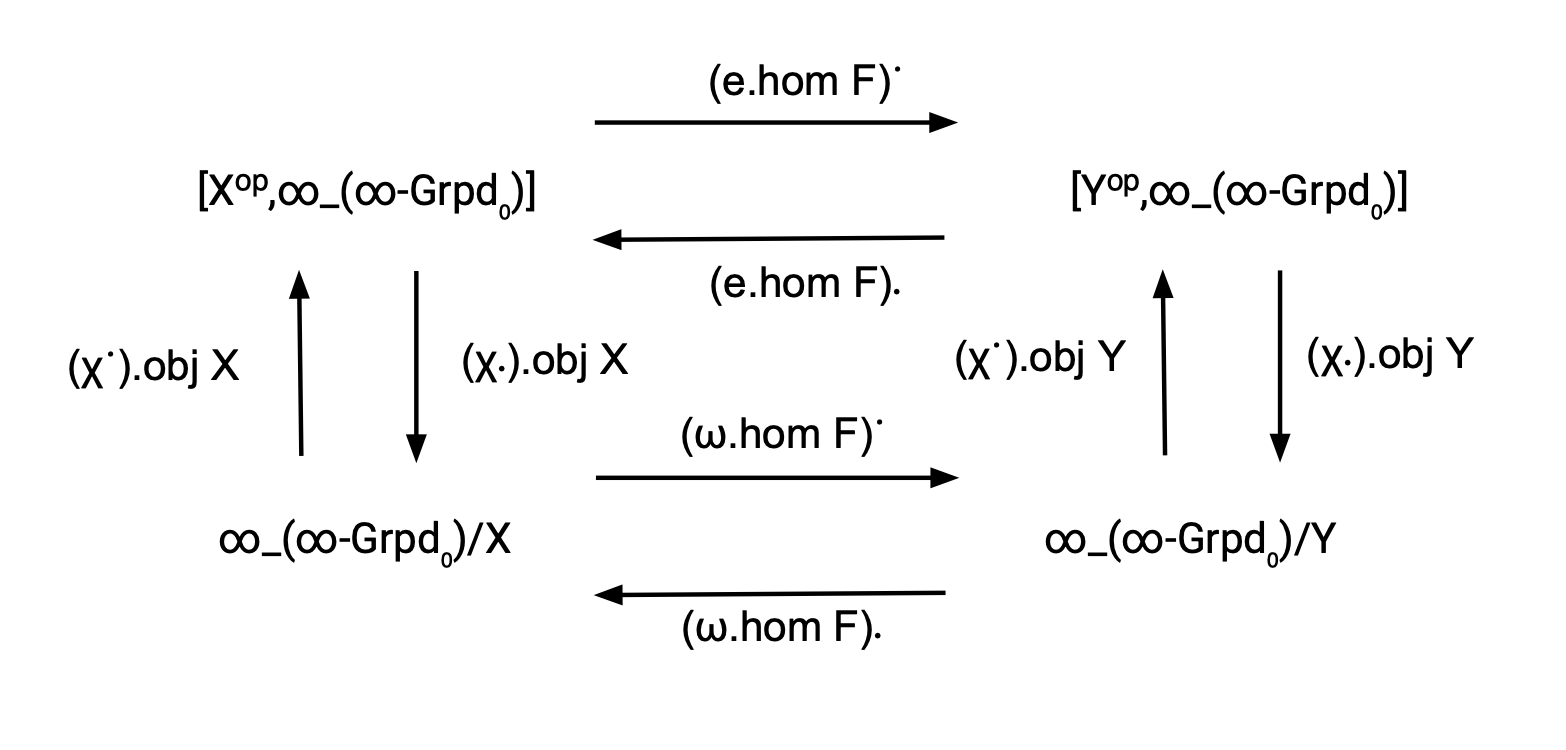
\includegraphics[width=0.9\textwidth]{ND00.png} \\
\end{center}

\ \\

\begin{center}
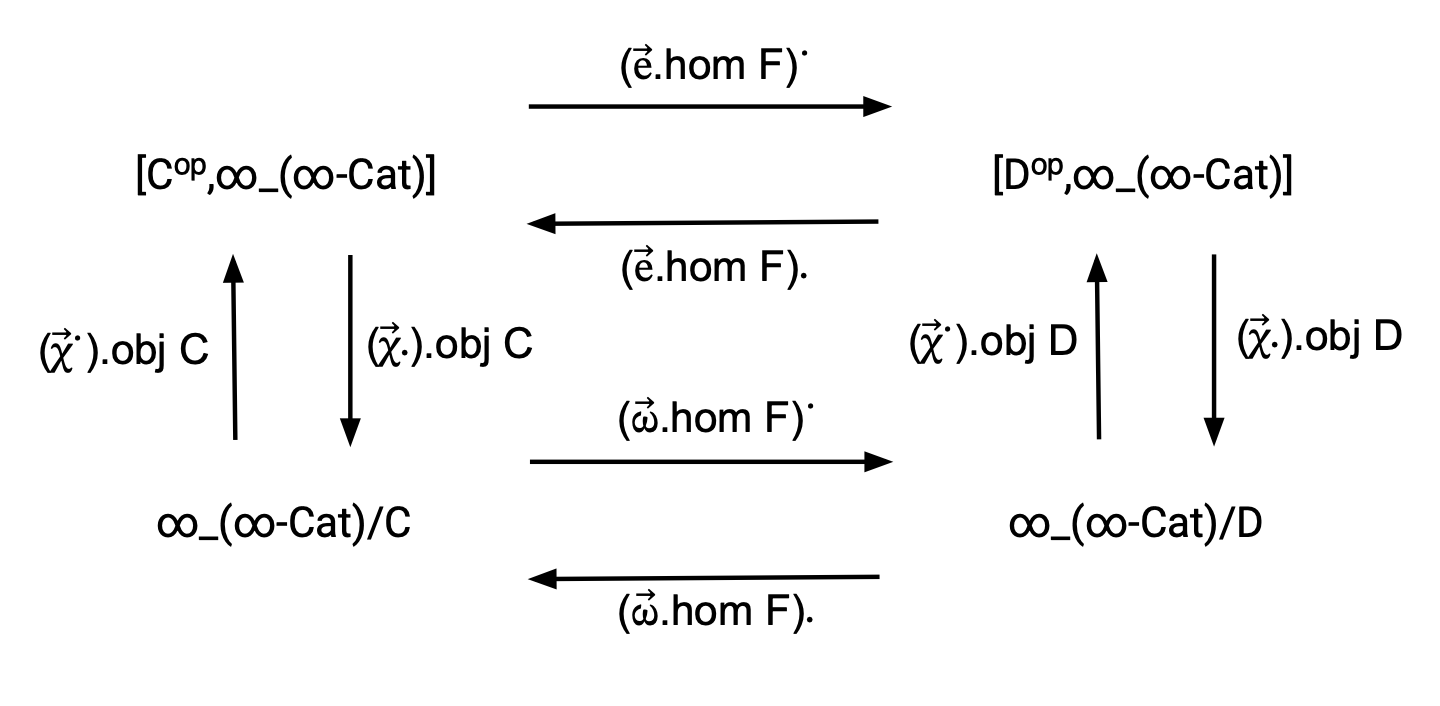
\includegraphics[width=0.9\textwidth]{ND10.png} \\
\end{center}

\ \\

\iffalse 
\begin{center}
\includegraphics[width=0.9\textwidth]{ND20.png} \\
\end{center}
\fi


\newpage


6 goals
6 structures

With these goals I want to create several ```remembrant''' adjunctions:

\iffalse
\begin{center}
Ω${}^{∞}$ : ∞-Cat ⇄ C-InfinityCategory ∞-Cat
\end{center}
Ω${}^{∞}$ 
\fi

\begin{enumerate}
\item γ⃗ γ⃡ γ
\item Σ⃗ Σ⃡ Σ
\item σ⃗ σ⃡ σ
\item Pullback of two homs and a single hom vs. a pushout of two products and a single product
\end{enumerate}


 



\begin{center}
o⃗ : (C : ∞-Cat) → ∞-Cat⁄C ⭢ OperadicPresheaf (O⃗.obj C)
\end{center}

defining B






\iffalse
% https://tikzcd.yichuanshen.de/#N4Igdg9gJgpgziAXAbVABwnAlgFyxMJZABgBpiBdUkANwEMAbAVxiRAB12cYAPHf4MgDCgJVxAarilAeEScA+gApJAWiF0cASgoBfEJtLpMufIRRkAjFVqMWbae3lLO3PgJXrAIgRDtu-djwEiAMzkFvTMrIggyAAi4lKyjrz8OMAKyqoaXnogGL5GgaTm1KHWEbb2Cc7JaeqabhVJwFFeFjBQAObwRKAAZgBOEAC2SGQgOBBIptQARjBgUEgBI8XhIHKA48CA9BuAKTtqAHQQUwBWAARCOll9gxPUY8PTs-OIi0VWK+uAjpB7Bydn3iCXQyeN3GiEmljCbHqAjkgEngQDrBLsABaDY4AMTUmm2IGoDDoMwYAAUDH5jCAGDBujhsSAZnMFsQ-gC7qMQQAmF4QiJQ5JyGAI5EDNEY97U2mPRaM-qA9ks5nLSFcRLQvlIlHozQiyVXUHAhYckocRWVFLw1WC9Wai5SpAy25A8EG9bbL5HY5RUUPelawFBWWIGVi+n6t5rT77V3uzRaIA
\begin{tikzcd}
{[Cop,infinitySUB(infinity-Cat)]} \arrow[d, "(χ${}_{\cdot}$).obj C", bend left] \arrow[rrr, "(e⃗.hom F)ॱ", bend left] &  &  & {[Dop,infinitySUB(infinity-Cat)]} \arrow[lll, "(e⃗.hom F)ॱ"] \arrow[d, "(χ${}_{\cdot}$).obj D", bend left]               \\
infinitySUB(infinity-Cat)⁄C \arrow[u, "(χ${}^{\cdot}$).obj C", bend left] \arrow[rrr, "\texttt{(ω⃗.hom F)}ॱ"]                   &  &  & infinitySUB(infinity-Cat)⁄D \arrow[lll, "(ω⃗.hom F)𛲔", bend left] \arrow[u, "(χ${}^{\cdot}$).obj D", bend left]
\end{tikzcd}

\fi

\begin{enumerate}
\item It is possible that the B lifts under slightly different conditions than those under which it is an endomorphism.
\item After use of the ∞-box, whose product is difficult, we can invert certain maps to obtain complexes. For this to work we need both biproducts and minus.
\item Not only must these spaces be based; B necessitates that they be A∞ or E∞ (plus some other thing about grouplike, for me).
\item After this we can consider the "free ???", but the product is a bit difficult.
\item [[ℕ,γ⃗], X]
\end{enumerate}


\begin{center}
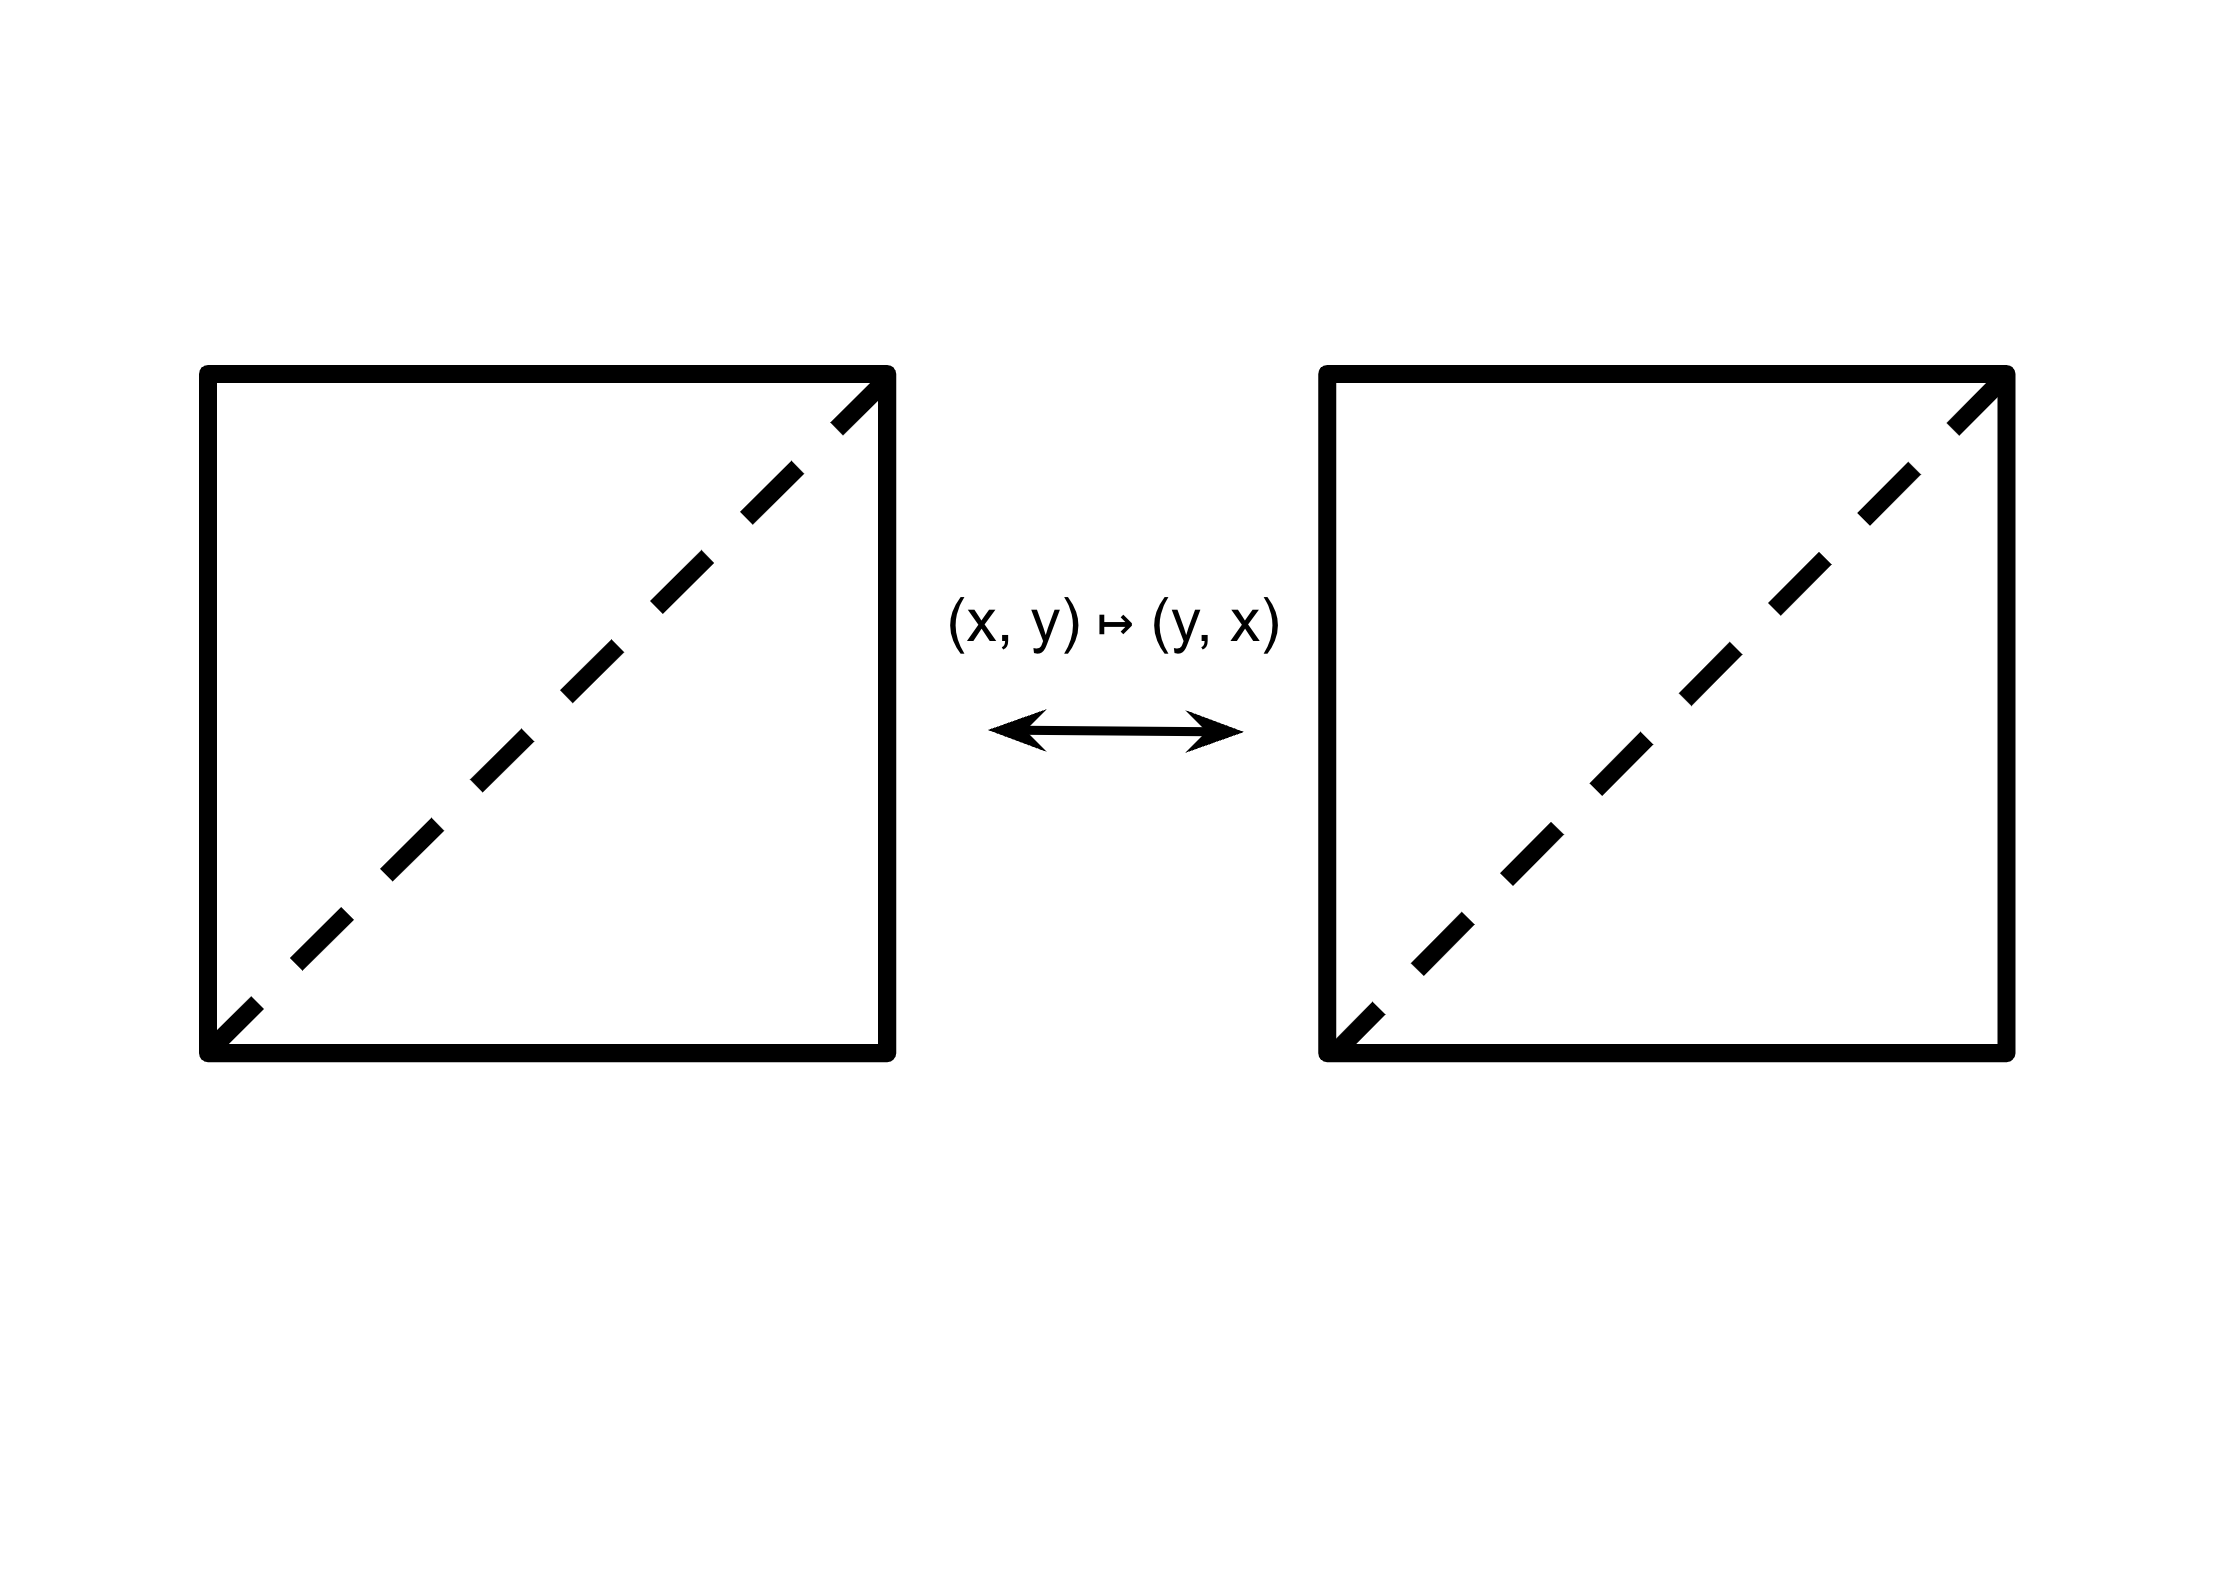
\includegraphics[width=0.5\textwidth]{littlesquaresA.png}
\end{center}
\ \\
\begin{center}
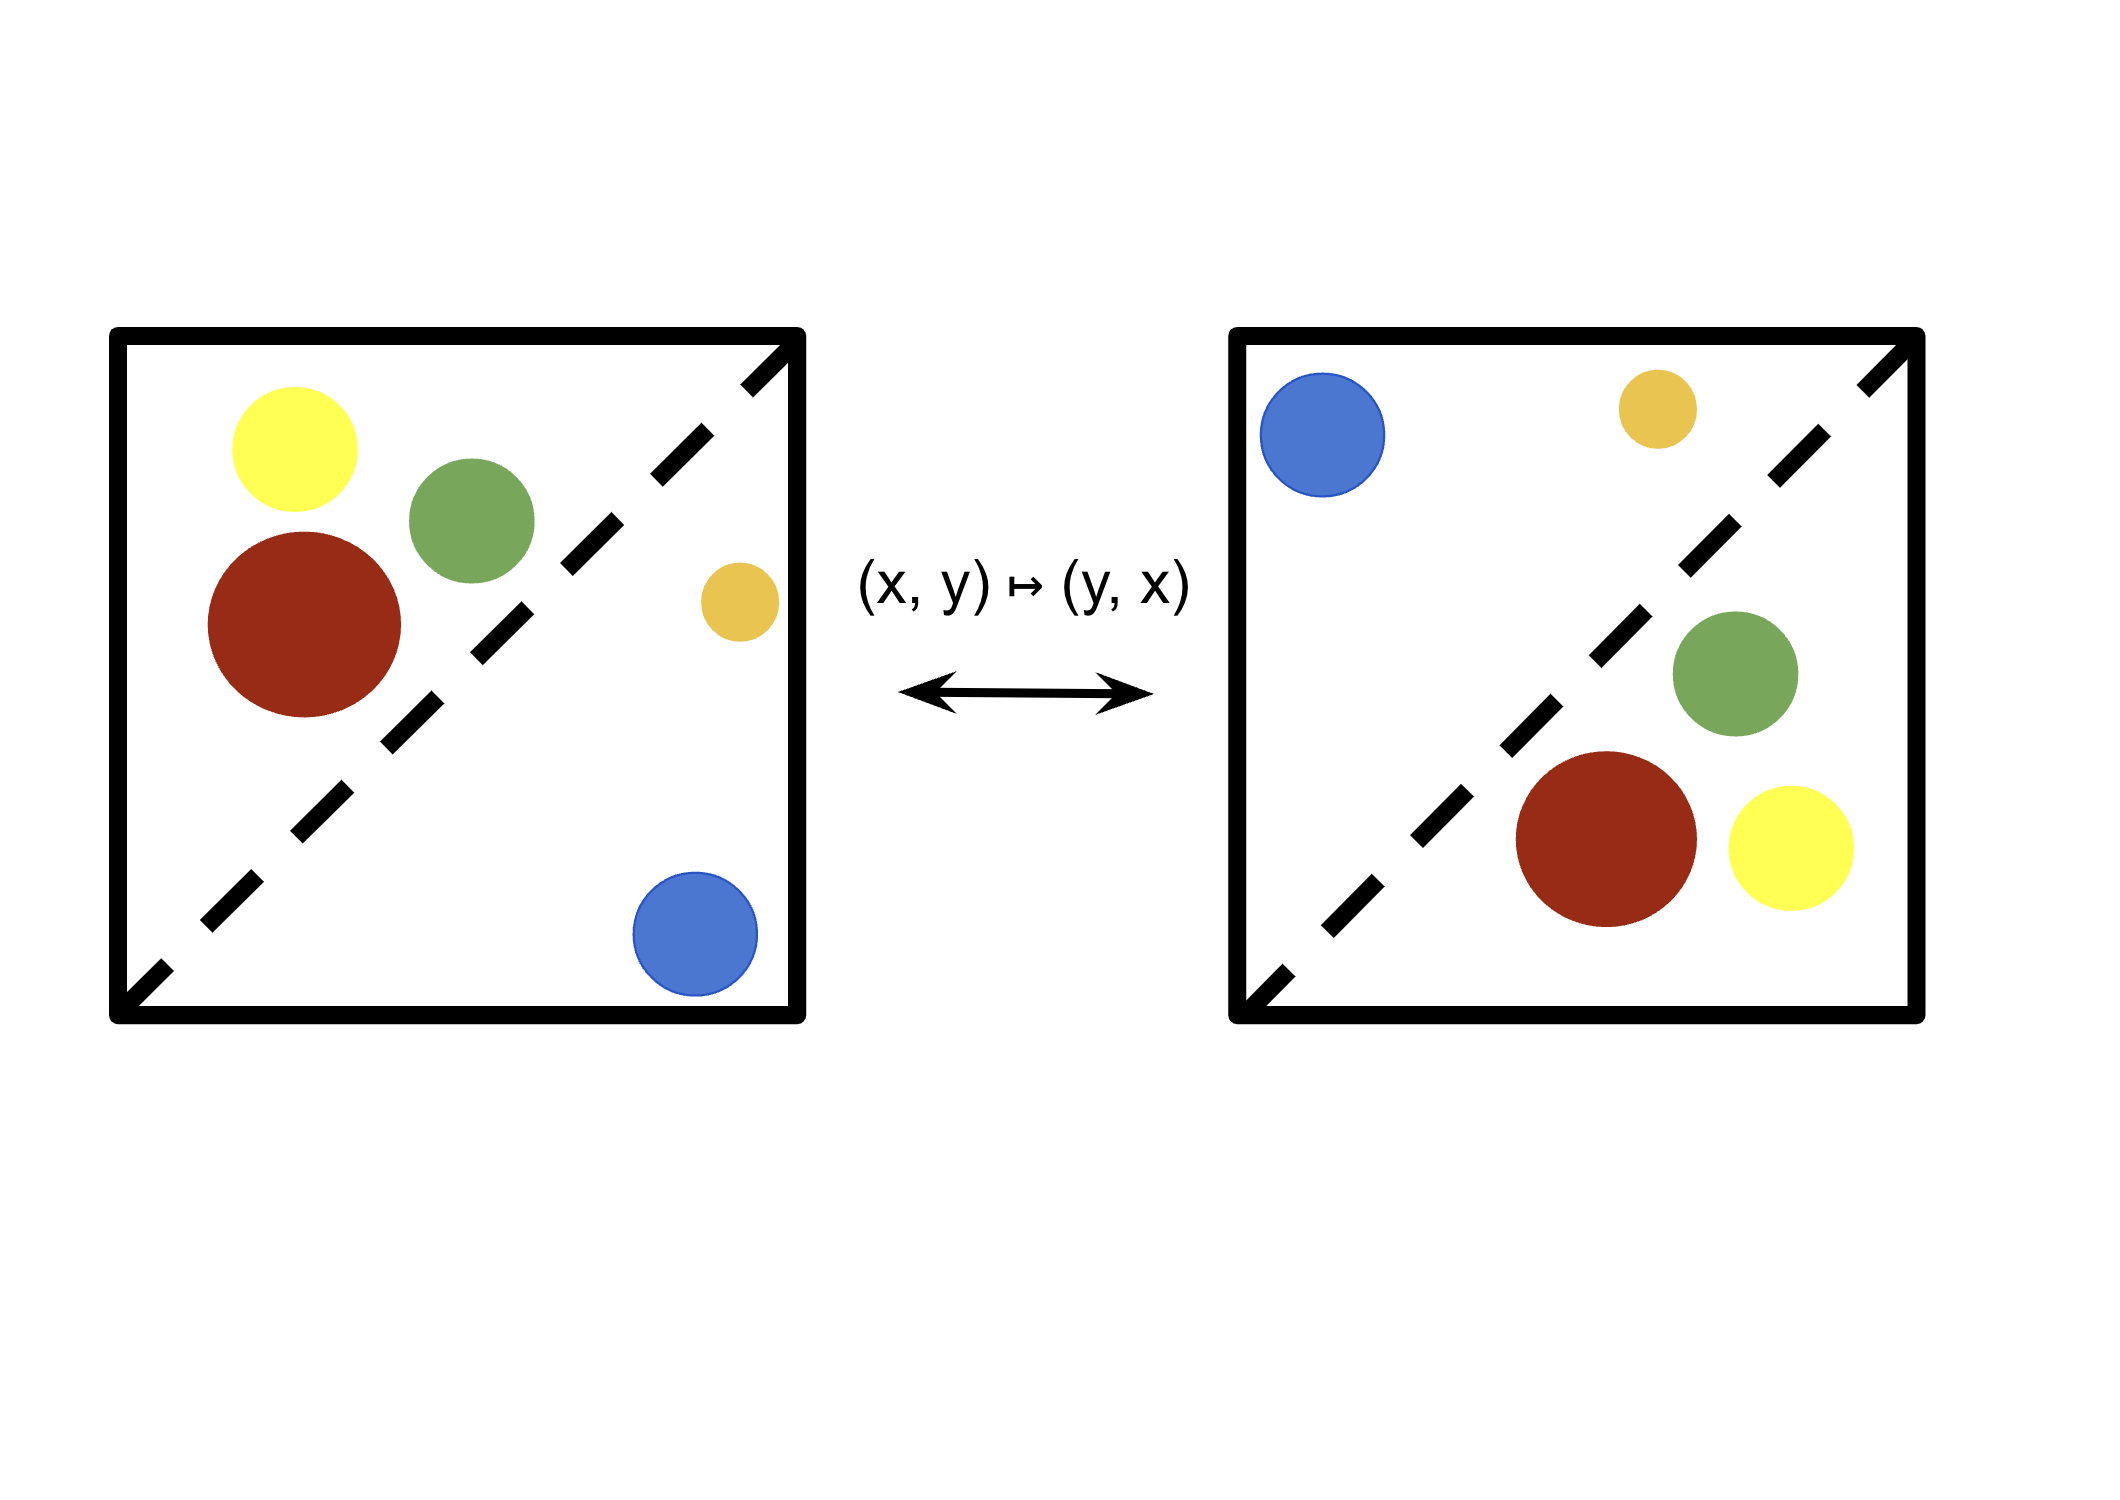
\includegraphics[width=0.5\textwidth]{littlesquaresB.png}
\end{center}


\iffalse
Iteration of the six operadic structures n times will give one of six versions of the little n-cubes operad ("operoid")
\fi




\newpage
\newpage
\section{Bibliography}


\begin{enumerate}
\item Serre, Jean-Pierre. "Homologie singulière des espaces fibrés. Applications." Annals of Mathematics 54, no. 3 (1951): 425-505.
\item
\end{enumerate}



\newpage 
\ \\
\ \\
\ \\
\ \\
\ \\               
\ \\
%LEAN: 
\begin{center}
\begin{tcolorbox}[width=5in,colback={white},title={\begin{center}\texttt{About the Author} \addtocounter{lcounter}{1}  \end{center}},colbacktitle=Yellow,coltitle=black]
Dean Young is a master's student at New York University, where he studies mathematics. \\
\begin{center}

\includegraphics[width=7.5cm,height=5cm]{about.jpg}
\end{center}
\end{tcolorbox}
\end{center}

\begin{center}
\begin{tcolorbox}[width=5in,colback={white},title={\begin{center}\texttt{About the Author} \addtocounter{lcounter}{1}  \end{center}},colbacktitle=Yellow,coltitle=black]
Jiazhen Xia is a graduate student at Zhejiang University, where he studies computer science. \\
\begin{center}

\includegraphics[width=7.5cm]{about2.jpg}
\end{center}
\end{tcolorbox}
\end{center}
\newpage
\ \\
\thispagestyle{empty}
\pagecolor{Yellow}



\end{document}







































